% For tracking purposes - this is V3.1SP - APRIL 2009
\documentclass{acm_proc_article-sp}
\usepackage{graphicx}
\usepackage{subfig} % for horizontal figures
\usepackage{amsmath}
\makeatletter
\let\@copyrightspace\relax
\makeatother
\newcommand*{\metafrac}[2]{\genfrac{}{}{0pt}{}{#1}{#2}} %fraction without line
\newcommand*{\bfrac}[2]{\genfrac{(}{)}{0pt}{}{#1}{#2}} %fraction without line

\begin{document}

\title{Hierarchical Control for Aircraft Electronic Power Systems}

\numberofauthors{2}
\author{
\alignauthor
Forrest N. Iandola\\
       \affaddr{University of California, Berkeley, USA}\\
       \email{forresti@eecs.berkeley.edu}
\alignauthor
Huy Vo\\
       \affaddr{University of California, Berkeley, USA}\\
       \email{huytbvo@eecs.berkeley.edu}
}

\maketitle
\begin{abstract}
As avionics and other aircraft electronics system increase in complexity, the task of controlling aircraft electronic power systems (EPS) becomes more challenging.
With this in mind, we present an aircraft EPS controller, or \emph{load management system (LMS)}, that guarantees safety while aiming to optimize quality of service metrics such as minimizing load shedding.
Our controller is a hierarchical load management system that combines an optimization-based model predictive LMS with a priority table based low-level LMS.
The fundamental contribution is in coupling the two controllers to work in a hierarchical fashion, where the optimization-based LMS looks forward and the low-level LMS guarantees safety in the short term.
Through simulations and numerical examples, we find that our hierarchical controller minimizes load shedding while always preserving safety in the aircraft EPS.
\end{abstract}

\keywords{avionics, model-predictive control, optimization, linear programming} 

\section{Introduction}
Aircraft Electrical Power Systems (EPS) are systems that provide power to critical loads (landing gear, navigation systems, etc.)
as well as non critical loads (cabin lights, coffee machine, etc). Above all else, an aircraft EPS controller must ensure that
power is constantly provided to all critical parts of the system. Since EPS are evolving into increasingly complex systems, EPS
controllers must become ``smarter''. We address the challenge of designing such a controller in this project. More specifically,
we contribute a Low Level Load Management System that closely monitors system status and ensures safety. We combine this
controller with an Optimzing Load Management System~\cite{mehdi} to obtain a Hierarchical Load Management System that is
both safe and optimal.

The rest of the paper is organized as follows.
In Sections~\ref{sec:overview} and~\ref{sec:related-work}, we give an overview of Aircraft EPS. %in order to provide the necessary background information for understanding the purposes of our controller. 
This is followed by a detailed discussion of an Optimizing Load Management System (Section~\ref{sec:optimizing-LMS}) and a Low Level Load Management System (Section~\ref{sec:LL-LMS}). 
After presenting these two controllers, we then show how to combine the two into a Hierarchical Load Management System. 
Finally, in Sections~\ref{sec:numerical-examples} and~\ref{sec:results}, we show that our hierarchical controller achieves safety where the Optimizing Load Management System would have been unable to and achieves optimality where the Low Level Load Management System cannot.

\section{Aircraft EPS Overview}
\label{sec:overview}
\begin{figure*}[htb]
  \centering
  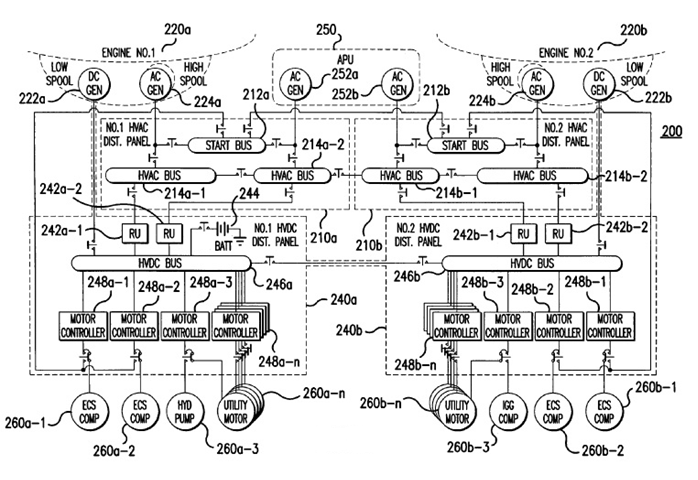
\includegraphics[width=\columnwidth]{figures/eps.png}
  \caption{\textbf{Single Line Diagram of Aircraft Electrical Power System} Detailed model of the EPS system from the Honeywell Patent used
  in this paper.}
  \label{fig:sld}
\end{figure*}
Figure~\ref{fig:sld} shows a detailed Single Line Diagram (SLD) of an aircraft EPS. The diagram shows AC and DC generators connected to the engines
as well as auxiliary power sources (APUs). These generators and power sources are responsible for providing power to the many critical and non-critical
AC and DC loads as well as power conversion equipments. Buses are responsible for distributing power from the generators to the loads. Electrical switches
called contactors route power from the generators to the buses. Current, voltage, and contactor sensors are used to monitor the status of the system. A
typical EPS controller consists of Generator Control Units (GCUs) and Bus Power Control Unit (BPCU). The GCU is used to regulate the power output of the
the generators as well as isolate failed generators. The BPCU is used to control the contactors thus making it responsible for routing power from the
generators to the load.

In this paper, we discuss \emph{load management systems (LMS)} that encompass the GCU and BPCU responsibilities such as load shedding and the assignment of generators to buses. 
The load shedding and generator assignments are actuated by the contactors, though we focus on the high-level control and assume there is an interface to convert our control instructions to contactor configurations.

Also, most of the examples in this paper use a system with the following configuration.
Each side of the aircraft has a bus, and the left-side and right-side buses each have a set of sheddable and nonsheddable tasks.
There are three generators--Generator 1 is part of the left-side engine, Generator 2 is part of the right-side engine, and the auxiliary power unit (APU) is generally used only when one or both of the main generators has failed.


\subsection{Load Shedding}
Aircraft EPS generally have two types of loads: sheddable and nonsheddable.
Examples of nonsheddable loads include navigation systems, electronic actuators, and other mission-critical devices.
Sheddable loads include the cabin lights, kitchen, and electrical outlets for passengers' laptop computers.
If an EPS power bus requires more power than the generators can provide, the LMS is responsible for disabling (shedding) some of the sheddable loads.

~\\
\section{Related Work}
\label{sec:related-work}
In typical aircraft EPS, the load management systems aim to ensure safety during unexpected system behavior.
Specifically, these systems require nonsheddable loads to remain powered at all times.\footnote{More precisely, nonsheddable loads must not be more unpowered for more than one cycle of the LMS. In practice, 50ms is a typical LMS sampling frequency.} %[or, maybe nonsheddable loads can be unpowered for up to 50ms while switching generators]
Therefore, if a generator fails, the EPS must shed loads and/or reallocate generators to buses such that no nonsheddable load becomes unpowered.
Typically, these systems rely on hard-coded priority tables for selecting loads to shed and for allocating generators to buses.

Beyond discussions of simply applying priority tables, perhaps the most closely related work in the Aircraft EPS community focuses on optimizing \emph{the EPS topology itself}~\cite{Chandrasekaran:2003, VanDriel:2006, Pinto:2010}. 
In contrast to these results, we focus on optimizing the control of load shedding and generator assignment of any given EPS topology, while also preserving safety.
An other related direction is the work by Xu et al.~\cite{xu:2012}, who proposes correct-by-construction design of load management systems.
While the work in~\cite{xu:2012} guarantees safety, it doesn't optimize for minimal load shedding or other similar metrics.

\section{Optimizing LMS}
\label{sec:optimizing-LMS}
LMS systems that are based purely on priority tables are very simplistic, allowing them to frequently sample the system. 
These LMS systems are thus more responsive to failures in the system.
However, pure priority table solutions tend to shed more loads than necessary, to use more generators than necessary, 
%[and be ill-defined in their tradeoffs between generator allocation and load shedding].
Toward resolving these issues, the control systems community recently designed a model-predictive Optimizing LMS for aircraft EPS~\cite{mehdi}.
The key insight in~\cite{mehdi} is to formulate the system requirements (e.g. the maximum power produced by each generator) as constraints in an linear optimization problem.
%Further,~\cite{mehdi} proposes an objective function such that solving the optimization problem produces a power system allocation using a minimal number of generators while also minimizing the total number and duration of loads that are shed. 
The Optimizing LMS minimizes an objective function comprised of three weighted vectors: load shedding preference, generator selection preference, and number of generators used.
The following expression gives a high-level view of the objective function in~\cite{mehdi}, where the weights can correspond with priorities in priority tables and $h$ is a time horizon:

$\int_t^{t+h} min(\bfrac{\text{sheddable}}{\text{loads}} * \text{\scriptsize \emph{weights}$_1$} +  \bfrac{\text{generator}}{\text{selection}} * \text{\scriptsize \emph{weights}$_2$} +  \bfrac{\metafrac{\text{\scriptsize \# of }}{\text{\scriptsize generators}}}{\text{\scriptsize used}})$

Notice the integral from time $t$ to time $t+horizon$. 
If the horizon=1, then we simply optimize the objective function for one system timestep.
However, if the horizon=10, then we do one call to the CPLEX~\cite{CPLEX} MILP solver to compute the optimal system configurations for 10 timesteps.
Batching several timesteps into one MILP call can reduce the overall computation time: using a 6-core Intel 3930K processor, optimizing 1 timestep takes an average of 350ms, while optimizing 10 timesteps takes an average of 500ms (so, 50ms per timestep in the batched configuration).

However, our {\emph receeding horizon} approach of doing a batched optimization at every 10 timesteps is not foolproof.
This is because, at time $t$, we can't perfectly predict the power loads or generator failures at timesteps in the range [$t+1$, $t+horizon$]. 
Therefore, instead of using live data from the load sensors, the Optimizing LMS uses historical data, averaged from previous flights that flew the same route using the same model of aircraft.
%However, the Optimizing LMS~\cite{mehdi} is not without shortcomings.
%Chiefly, the Optimizing LMS is computationally expensive (0.5s for 10 timesteps of optimization in CPLEX on an Intel 3930K processor).
%[Discuss receding horizon and the need for historical data]
Since the Optimizing LMS relies on historical data, it may produce unsafe allocations that use a broken generator or operate above the generator power caps.
Thus, it is potentially unsafe to use Optimizing LMS to control the electronics in a real airplane. 
However, as we will see later in the paper, the Optimizing LMS can be effective if it is coupled with a fail-safe Low Level LMS.

\section{Low Level LMS (LL-LMS)}
\label{sec:LL-LMS}
\begin{table}[t]
\caption{\textbf{Load Priority Table Example, NS = nonsheddable, S = sheddable} 
Loads lower in the list have lower priority while loads higher up in the list have
higher priority. LL-LMS will shed load starting at the lower end of the list.}
\label{T:shed}
\centering
\begin{tabular}{c|cc}
 NS loads (W) & S loads (W) & Shed priority \\ \hline
1000 & 1000 & 1 \\
1000 & 5000 & 2 \\
500 & 2000 & 3 \\
5000 & 2000 & 4 \\
1000 & 1000 & 5 \\
1000 & 5000 & 6 \\
2000 & 1000 & 7 \\
5000 & 2000 & 8 \\
500 & 2000 & 9 \\
2000 & 1000 & 10 \\ \hline
\end{tabular}
\end{table}

\begin{table}[t]
\caption{Priority table for allocating generators to buses.}
\label{T:generator-priority}
\centering
\begin{tabular}{c|cc}
 Priority & Left bus & Right bus \\ \hline
1 (most preferred) & Generator 1 & Generator 2 \\
2 ~(mid preferred) & Generator 2 & Generator 1 \\
3 (least preferred) & APU & APU \\ \hline
\end{tabular}
\end{table}

\subsection{LL-LMS Overview}
As the name suggests, the LL-LMS serves as a simple, fail-safe controller in an aircraft power system.
Above all else, the LL-LMS must guarantee safe aircraft EPS operation.\footnote{For the purposes of this paper, we consider the following safety requirements: no load remains unpowered for more than 50ms, loads are not connected to unpowered generators, and no generator is connected to loads whose power request exceeds the power rating of the generator.}
Briefly, the LL-LMS uses various sensors to frequently sample the state of the system. It then uses its sensor readings along with its
priority tables, such as the one in Table~\ref{T:shed}, to produce a safe system configuration.

\subsection{LL-LMS Implementation}
Every cycle, the LL-LMS reads sensors to collect data on generator status and power requests on all the nonsheddable and sheddable loads. 
The LL-LMS first filters out unhealthy generator tables and then uses its generator priority table to determine which of the remaining healthy generators it should use to power the system. 
Once it has determined what generator to use, the LL-LMS will then determine how much load it has to shed. 
It first sums up power requests of all the loads (sheddable and nonsheddable) on each bus. 
It then determines if the generator for each of the buses are able to power all of the loads. 
If the power request is more than a generator can provide, the LL-LMS will start shedding sheddable loads starting at the load with the lowest priority. 
This simple generator selection and load shedding scheme ensure that the LL-LMS can quickly arrive at a safe system configuration.

%% This section presents a Low-Level LMS (LL-LMS) similar to the controllers discussed in Section~\ref{sec:related-work}.
%% The key goal (and perhaps the only) goal of this load management system is to preserve safety if workloads change or if  generators fail.
%% Therefore, using a pre-defined priority table of generator assignments and loads to shed, our LL-LMS sheds loads until the power requirement is within the generator's power budget.

%[TODO: 4-line pseudo-code for how we apply priority tables]


\section{Hierarchical LMS}
In this section, we begin with an overview of our Hierarchical LMS.
Then, we explain how we modify the Optimizing LMS (from Section~\ref{sec:optimizing-LMS}) and LL-LMS (from Section~\ref{sec:LL-LMS}) to accommodate our hierarchical strategy.
Finally, at the end of this section, we describe the hierarchical strategy for communication between the LL-LMS and Optimizing LMS.

\subsection{Overview}
Recall that the goal of our work is not to design an LMS that is safe OR optimal. 
Rather, we want to build an LMS that is both safe AND optimal. 
To this end, we propose a hierarchical LMS that achieves the best of both worlds by combining an optimizing LMS with a low level LMS. The Optimizing LMS periodically, though at a slow rate, receives the the generator status and produces a system configuration that is optimal in terms of historical workload data. 
%More specifically, the Optimizing LMS checks the status of the generators and solves the optimization problem detailed in Section~\ref{sec:optimizing-LMS}. 
The LL-LMS collects the advice from the Optimizing LMS and determines whether or not the advice is safe. 
If the advice is safe, the LL-LMS will actuate the system based on the Optimizing LMS's advice. 
Otherwise, the LL-LMS will fall back to its priority table. 
Because failures are rare, the LL-LMS will spend most of the time actuating the system based on the Optimizing LMS's advice. 
This Hierarchical LMS is optimal because the Optimizing LMS is optimal and is safe because the LL-LMS is safe.

\subsection{Modifications to Optimizing LMS}
Instead of having the Optimizing LMS system read the sensors directly as it would in a system that relies solely on an Optimizing LMS, it will instead receive its system status information from the LL-LMS. 
%This communication strategy saves on communication links between sensors and the Optimizing LMS and reuses the communication link between the LL-LMS and the Optimizing LMS. 
This communication strategy allows the LL-LMS to have the final word on selecting a system configuration.
%We also use the Optimizing LMS to perform live optimizations of the system. 
%That is, 
%smaller receding horizon. 
%Most importantly, this implementation is resilient to generator failures. 
Further, instead of solving one large offline optimization problem use a receding horizon that covers the entire flight, we have the Optimizing LMS periodically solve a batch of system configuration optimizations using small receding horizon.
%Previously, the Optimizing LMS would be completely oblivious to generators that fail mid-flight. 
With this modification, the Optimizing LMS will eventually see that there is a generator failure and reoptimize for the new topology.

\subsection{Modifications to LL-LMS}
The LL-LMS will now receive advice from the Optimizing LMS in addition to its other functionalities detailed in Section~\ref{sec:LL-LMS}. The LL-LMS will then
check to see that the Optimizing LMS's advice is safe. Specifically, the LL-LMS will check that the Optimizing LMS did not recommend the use of a failed generator and that
the Optimizing LMS has shed enough loads so that no generator is overloaded. In the case that the Optimizing LMS recommended the use of a failed generator, the LL-LMS
will use the next best generator according to its priority table and perform the appropriate load shedding. In the case that Optimizing LMS advice would cause a
generator overload, the LL-LMS will shed additional loads so that the power request on the bus is under the corresponding generator's power rating.

\subsection{Hierarchical LMS Implmentation}

\begin{figure*}[hp]
  \centering
  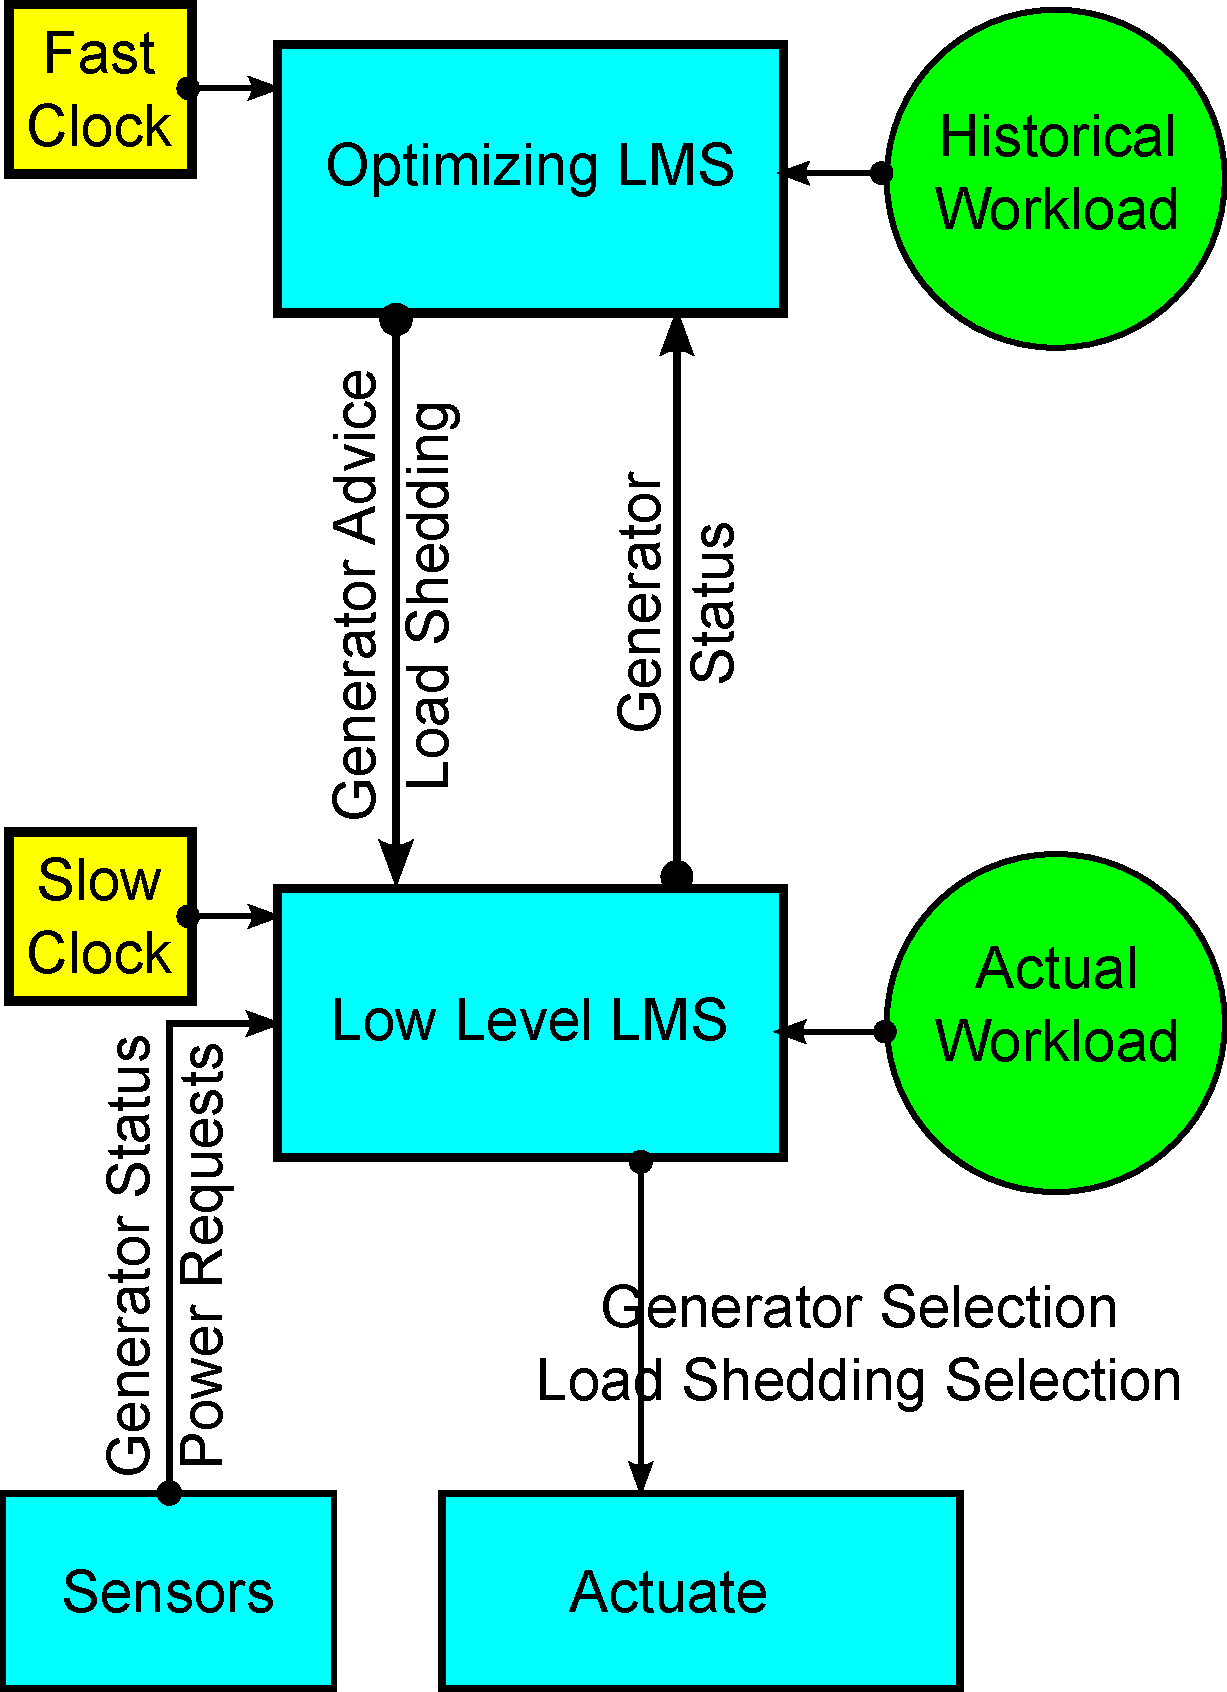
\includegraphics[width=0.75\textwidth]{figures/H-LMS.pdf}
  \caption{\textbf{Hierarchical LMS Block Diagram} The Optimizing LMS and the LL-LMS runs at different rates. The Optimizing LMS no longer communicates directly with the EPS sensors
and actuators. The LL-LMS is the last level of controller and communicates directly with the EPS sensors and actuators. The LL-LMS periodically sends
generator status to the Optimizing LMS which the Optimizing LMS uses in its next iteration. The Optimizing LMS produces advice that it sends to the LL-LMS. Whether or not the Optimizing LMS's
advice is ever actuated on is left to the discretion of the LL-LMS.}
  \label{fig:H-LMS}
\end{figure*}

Figure~\ref{fig:H-LMS} shows the block diagram of our hierarchical controller. 
The different clocks fed into the two controllers indicate that the two controllers operate at different frequencies. 
More specifically, the LL-LMS operates at a high frequency, fast enough to ensure that the system is not in an unsafe configuration for more than 50 ms. 

On the other hand, the Optimizing LMS runs at a much slower rate due to the complexity of the optimization problem.
Recall from Section~\ref{sec:optimizing-LMS} that the Optimizing LMS can optimize over a horizon of 10 timesteps every 500ms. 
Therefore, we set the LL-LMS to sample at a frequency of 50ms (controlled by the fast clock in Figure~\ref{fig:H-LMS}), we set the Optimizing-LMS to use a horizon of 10 timesteps, and thus the Optimizing-LMS gives a batch of advice to the LL-LMS every 500ms.

At each 500ms interval, the Optimizing LMS produces a set of 10 timesteps worth of advice (generator usage recommendations as well as load shedding configurations) that can the LL-LMS can use until the next Optimizing LMS cycle. 
Notice that there is an arrow going from the the LL-LMS to the Optimizing LMS because the LL-LMS is responsible for providing the Optimizing LMS with information of the status of the generators. 
The generator usage and load shedding that the LL-LMS will actuate on will be either the advice provided by the Optimizing LMS
if it is safe or the configuration determined by the LL-LMS's priority table if the Optimizing LMS's advice is unsafe.

\section{Numerical Examples}
\label{sec:numerical-examples}
In the following numerical examples, we show how Hierarchical LMS harnesses the Optimizing LMS and LL-LMS to handle interesting load shedding situations and failure scenarios.
For simplicity, let each of these examples be limited to the loads in the left side bus.
Further, to keep the examples simple, we just look at sheddable loads powered by a generator with a power cap of 100,000W.
In practice, aircraft EPS typically have a mix of sheddable and nonsheddable loads.

\subsection{Example: No failures or power spikes}
\label{sec:load-shedding-example}
We now present an example that illustrates how the Optimizing LMS manages to shed fewer loads than the LL-LMS. 
In this example, there are no generator failures or power spikes (the historical data matches the live data), so the Hierarchical LMS would use the advice for the Optimizing LMS.

\begin{tabular}{c|cc}
Sheddable loads (W) & Shed priority \\ \hline
60,000 & 1 (least preferred to shed) \\
60,000 & 2 (middle priority to shed) \\ 
40,000 & 3 (most preferred to shed) \\ \hline
\end{tabular}

When presented with this workload, the LL-LMS purely applies the priority table, without any optimization or branch-and-bound to investigate ideal combinations of tasks to shed. 
Thus, while simply shedding Load 2 would be sufficient to get system under its power cap, the LL-LMS walks up the priority table and sheds Loads 2 and 3.

In contrast, the Optimizing-LMS views the priorities as weights instead of precedence constraints. 
Therefore, the Optimizing-LMS sheds Load 2 and doesn't shed Load 3. 
%This is one type of situation where the Optimizing-LMS [wins] over the LL-LMS. 
Thus, the Optimizing LMS reduces load shedding compared to the LL-LMS.
The Optimizing-LMS produces safe results in this example, so the Hierarchical LMS shares the Optimizing-LMS's reduction in load shedding.

\subsection{Example: LL-LMS Preserves Safety \\ during Power Spike}
\label{sec:power-spike-example}
In this example, we show how the Hierarchical LMS preserves safety when the live workload data demands more power than the historical data predicts. 
At Timestep 1 in the following tables, the live data matches the historical data, and the Optimizing LMS provides safe advice.
However, Timestep 2 has a power spike in Load 3 that is not anticipated in the historical data. 
Relying on the Optimizing-LMS alone at Timestep 2 would result in an unsafe configuration, where 120,000W is draw, while the generator can only produce 100,000W.
Fortunately, the LL-LMS in our Hierarchical controller observes the Load 3 power spike in real-time, and it sheds Load 3 to maintain safety, thus maintaining a total power draw of 80,000W, which is within the generator's 100,000W power cap.

~\\ %skip a line
Timestep 1 (live data matches historical data):\\
\begin{tabular}{c|cc}
Sheddable loads (W) & Shed priority \\ \hline
40,000 & 1 (least preferred to shed) \\
40,000 & 2 (middle priority to shed) \\ 
{\bf 20,000} & 3 (most preferred to shed) \\ \hline
\end{tabular}

Timestep 2 (historical data): \\
\begin{tabular}{c|cc}
Sheddable loads (W) & Shed priority \\ \hline
40,000 & 1 (least preferred to shed) \\
40,000 & 2 (middle priority to shed) \\ 
{\bf 20,000} & 3 (most preferred to shed) \\ \hline
\end{tabular}

Timestep 2 (live data): \\
\begin{tabular}{c|cc}
Sheddable loads (W) & Shed priority \\ \hline
40,000 & 1 (least preferred to shed) \\
40,000 & 2 (middle priority to shed) \\ 
{\bf 40,000} & 3 (most preferred to shed) \\ \hline
\end{tabular}

\subsection{Example: LL-LMS handles generator failure}

We use the following loads for all timesteps in this example: \\
\begin{tabular}{c|cc}
Sheddable loads (W) & Shed priority \\ \hline
40,000 & 1 (least preferred to shed) \\
40,000 & 2 (middle priority to shed) \\ 
20,000 & 3 (most preferred to shed) \\ \hline
\end{tabular}

As with our other examples in this section, we're concentrating on the left side bus, which is powered by the left generator (labeled as Generator 1).
Now, let Generator 1 fail at Timestep 2. 
If we solely relied on the Optimizing-LMS, the left-side bus would continue to be powered by the (broken) Generator 1 during the time that the Optimizing-LMS reruns the optimization for the new topology.
However, in the Hierarchical LMS, the LL-LMS steps in at the time of the generator failure and reassigns the left side bus to Generator 2 (following the priorities in Table~\ref{T:generator-priority}).\footnote{Notice in Table~\ref{T:generator-priority} that Generator 2 is preferred over the APU in the left side bus's priority table. This is because, in addition to handling generator failures, the generator assignment is also valuable in situations with low power demand. For example, when taxiing around the airport, the aircraft can often conserve fuel by only using one generator. A byproduct of this policy is that, in the event of a generator failure, the priority table prefers to run the entire aircraft on a single generator instead of using the APU.}
Some loads may need to be shed to run the whole system off of generator 2.
However, so long as the nonsheddable loads in both buses are within the power cap of generator 2 then, both side buses remain powered. 
Then, the Optimizing-LMS is alerted of the generator failure in its next optimization run. 
When the MILP solver finishes solving the optimization problem, the Optimizing-LMS reports a new configuration to the LL-LMS. 
This configuration would include assigning the APU to power the left bus.


\section{Experimental Results}
In this section, we simulate a number of system configurations that demonstrate the Hierarchical LMS's combination of safe operation and optimization where feasible.
The examples in Section~\ref{sec:numerical-examples} provide the intuition for some of these simulation experiments, and the simulations help to further validate the Hierarchical LMS.
Our simulation setup is constructed in Matlab and Simulink, and the Optimizing LMS uses CPLEX to solve its optimization problem.

\label{sec:results}
\begin{figure}[htb]
  \centering
  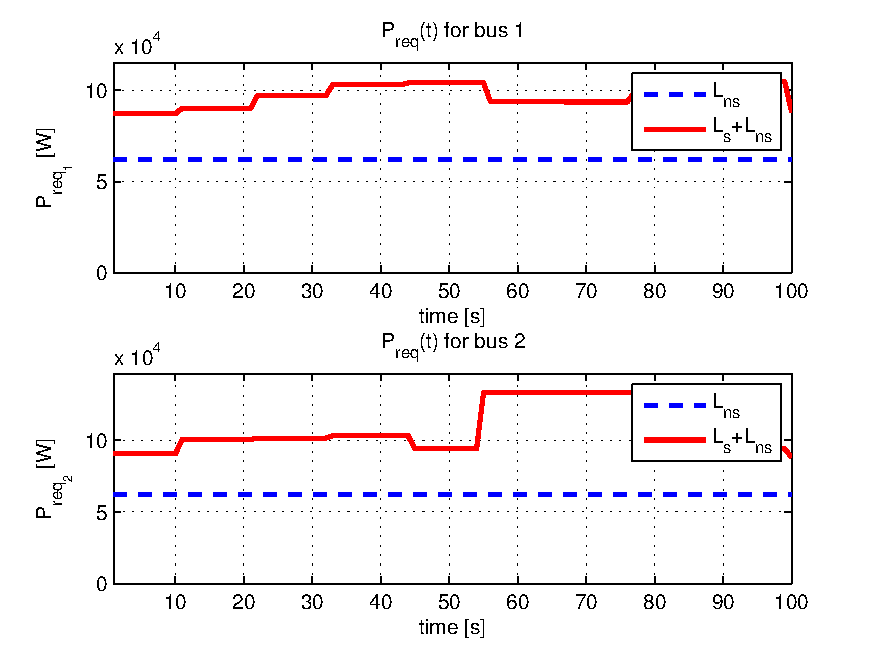
\includegraphics[width=\columnwidth]{figures/preqnofail}
  \caption{\textbf{Power Request}
  Historical data of power request on Bus 1 and Bus 2 for time 0
  to 100. Notice the spikes in power usage on Bus 2 that pulls the
  request over 100000 Watts, well over the power rating of the generators.
  Load shedding is a must during those intervals.}
  \label{fig:preqnofail}
\end{figure}

\subsection{No Failures}
\begin{figure*}[hp]
  \centering
  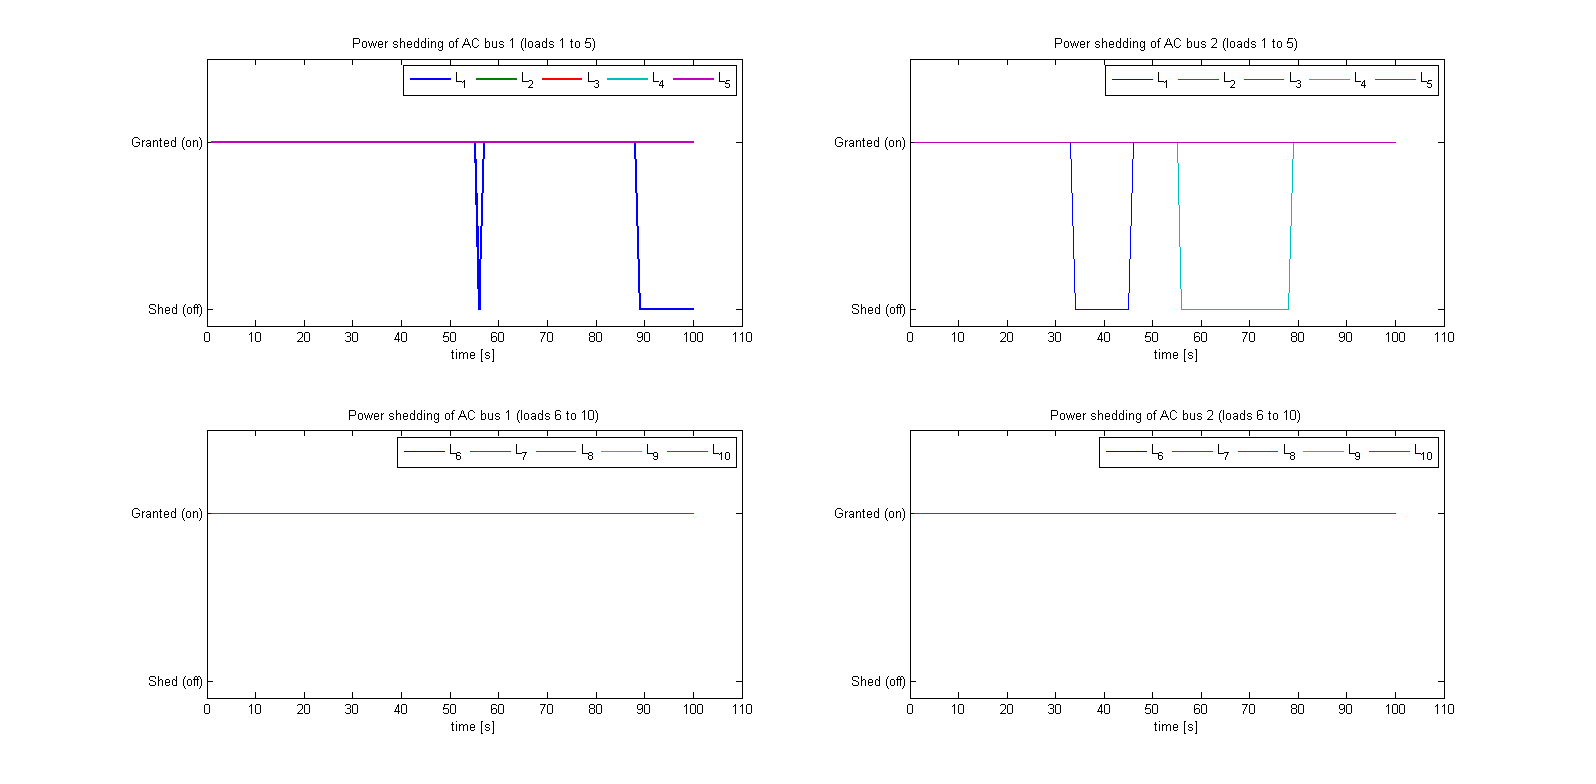
\includegraphics[width=\textwidth]{figures/lshlnofail}
  \caption{\textbf{Optimizing LMS Load Shedding} Notice the long
  period of load shedding around the power usage spikes.}
  \label{fig:lshlnofail}
\end{figure*}
\begin{figure*}[hp]
  \centering
  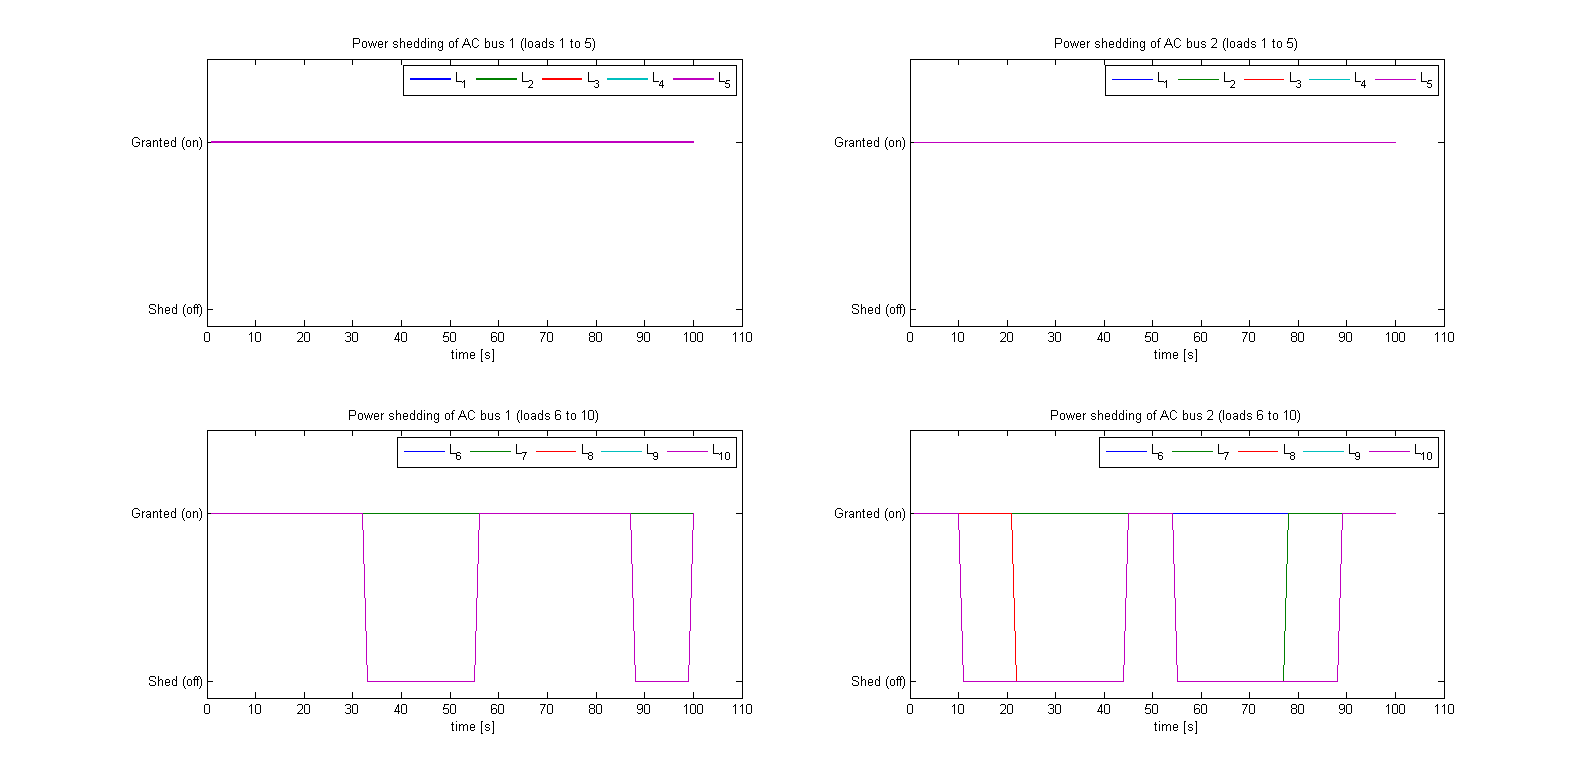
\includegraphics[width=0.9\textwidth]{figures/lsllnofail}
  \caption{\textbf{LL-LMS Load Shedding} Notice that the 
  LL-LMS sheds much more load than the Optimizing LMS.}
  \label{fig:lsllnofail}
\end{figure*}

We begin by simulating the case when there are no power
generator failures in the system using the power usage profile shown in
Figure~\ref{fig:preqnofail}. 
In other words, the real power usage profile (Figure~\ref{fig:preqnofail}) is given to the Optimizing LMS and LL-LMS without any perturbations.
Notice that Bus 1 requests more than 100,000 Watts
between time 30 and 60 and again around time 90. Bus 2, on the other hand,
has a massive power usage between time 50 and 80. We wanted to see how the
Optimizing LMS and the LL-LMS responds to this scenario in isolation. 
%Our results are in Figure~\ref{fig:lshlnofail} and Figure~\ref{fig:lsllnofail}.
Comparing the results, we can see that the LL-LMS will shed a much larger
number of loads (Figure~\ref{fig:lshlnofail}) than the the Optimizing LMS (Figure~\ref{fig:lsllnofail}). 
In particular, the LL-LMS sheds exclusively from loads 6-10 due to the configuration of the priority table.
%However, the Optimizing LMS however is much smarter. 
However, the Optimizing LMS sheds fewer loads, due to the intuition described in the numerical example in Section~\ref{sec:load-shedding-example}.
Specifically, the Optimizing LMS reduces the number of loads shed by shedding loads by cherry-picking weighted loads throughout the priority table instead of shedding all low-priority loads before shedding high-priority loads.
Since the system in this example experienced no generator failures or unexpected power spikes, running the system with only the Optimizing LMS or with the Hierarchical LMS produces the same result (Figure~\ref{fig:lshlnofail}).

\subsection{Generator Failure}
Now, we investigate how our Hierarchical LMS system responds to spontaneous generator failures. 
To this end, we simulated the case when generator 2 (which was powering the right bus) would fail at time 45. 
Obviously, if the Optimizing LMS were to run in isolation, it would leave the system unpowered from time 45 to 50. 
Figure~\ref{fig:lsllonefail} shows what would happen if the LL-LMS were to run in  isolation. 
Starting at time 45, the LL-LMS sees that generator 2 has failed and it has switched to using generator 1 to power both buses according to its priority table. 
In order to stay under generator 1's power rating, the LL-LMS sheds a large number of loads on the second bus. Figure~\ref{fig:lsolonefail} shows what would happen in a combined Optimizing LMS LL-LMS system. 
The Optimizing LMS produces advice to be used from time 40 to 50. 
Unfortunately, there is no way for the Optimizing LMS's advice to be aware of the failure at time 45. 
So, while the advice from time 40 to 44 is optimal and safe, the advice from 45 to 49 is unsafe. 
The LL-LMS is able to see this failure at time 45 and kicks in, ignoring the unsafe advice from the Optimizing LMS. 
This behavior is observed in Figure~\ref{fig:lsolonefail} where from time 45 to 49, a large number of loads are shed. 
(Given the priorities in Table~\ref{T:generator-priority}, the LL-LMS prefers to use generator 1 instead of the APU to power the right bus.)
Then at time 50, the Optimizing LMS reoptimizes by turning on the APU.
Notice the difference in the number of loads shed onward after time 50 in Figure~\ref{fig:lsllonefail} and Figure~\ref{fig:lsolonefail}.

\begin{figure*}[hp]
  \centering
  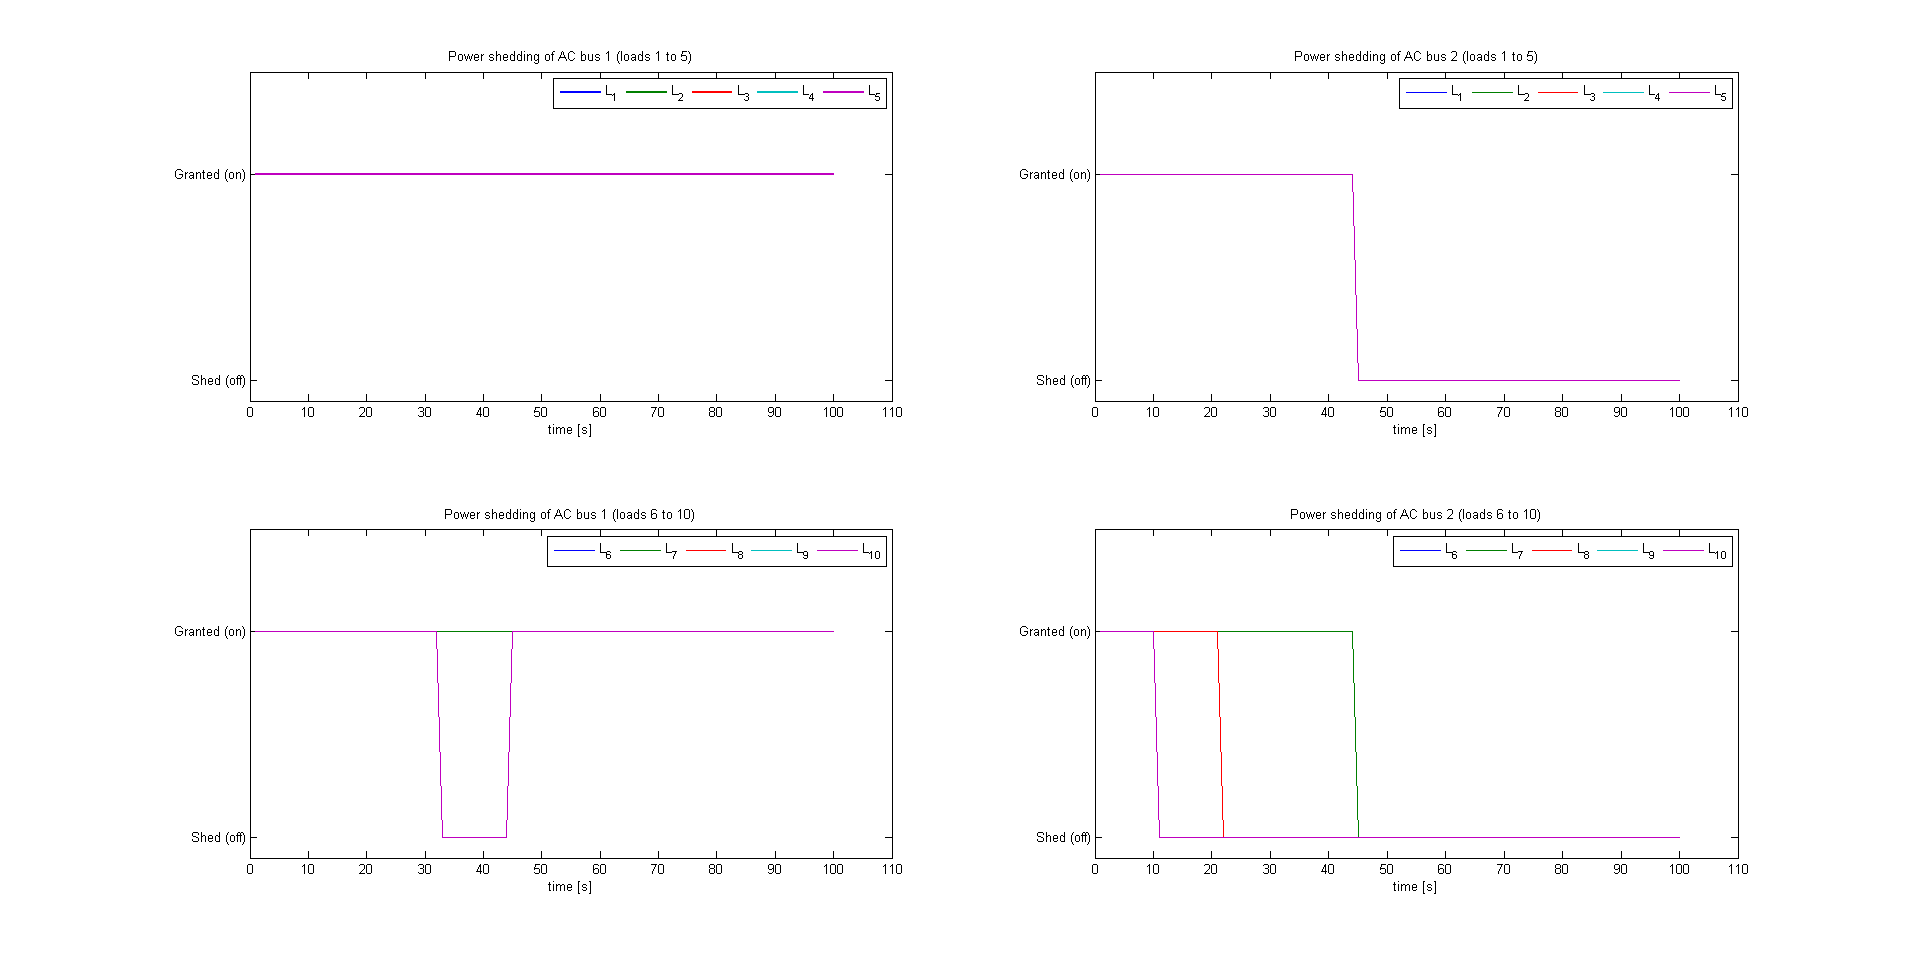
\includegraphics[width=0.9\textwidth]{figures/lsllonefail}
  \caption{\textbf{LL-LMS Load Shedding -- One Generator Failure}. Notice
  the large amount of loads shedded in order to keep power usage below the power rating
  of generator 1.}
  \label{fig:lsllonefail}
\end{figure*}
\begin{figure*}[hp]
  \centering
  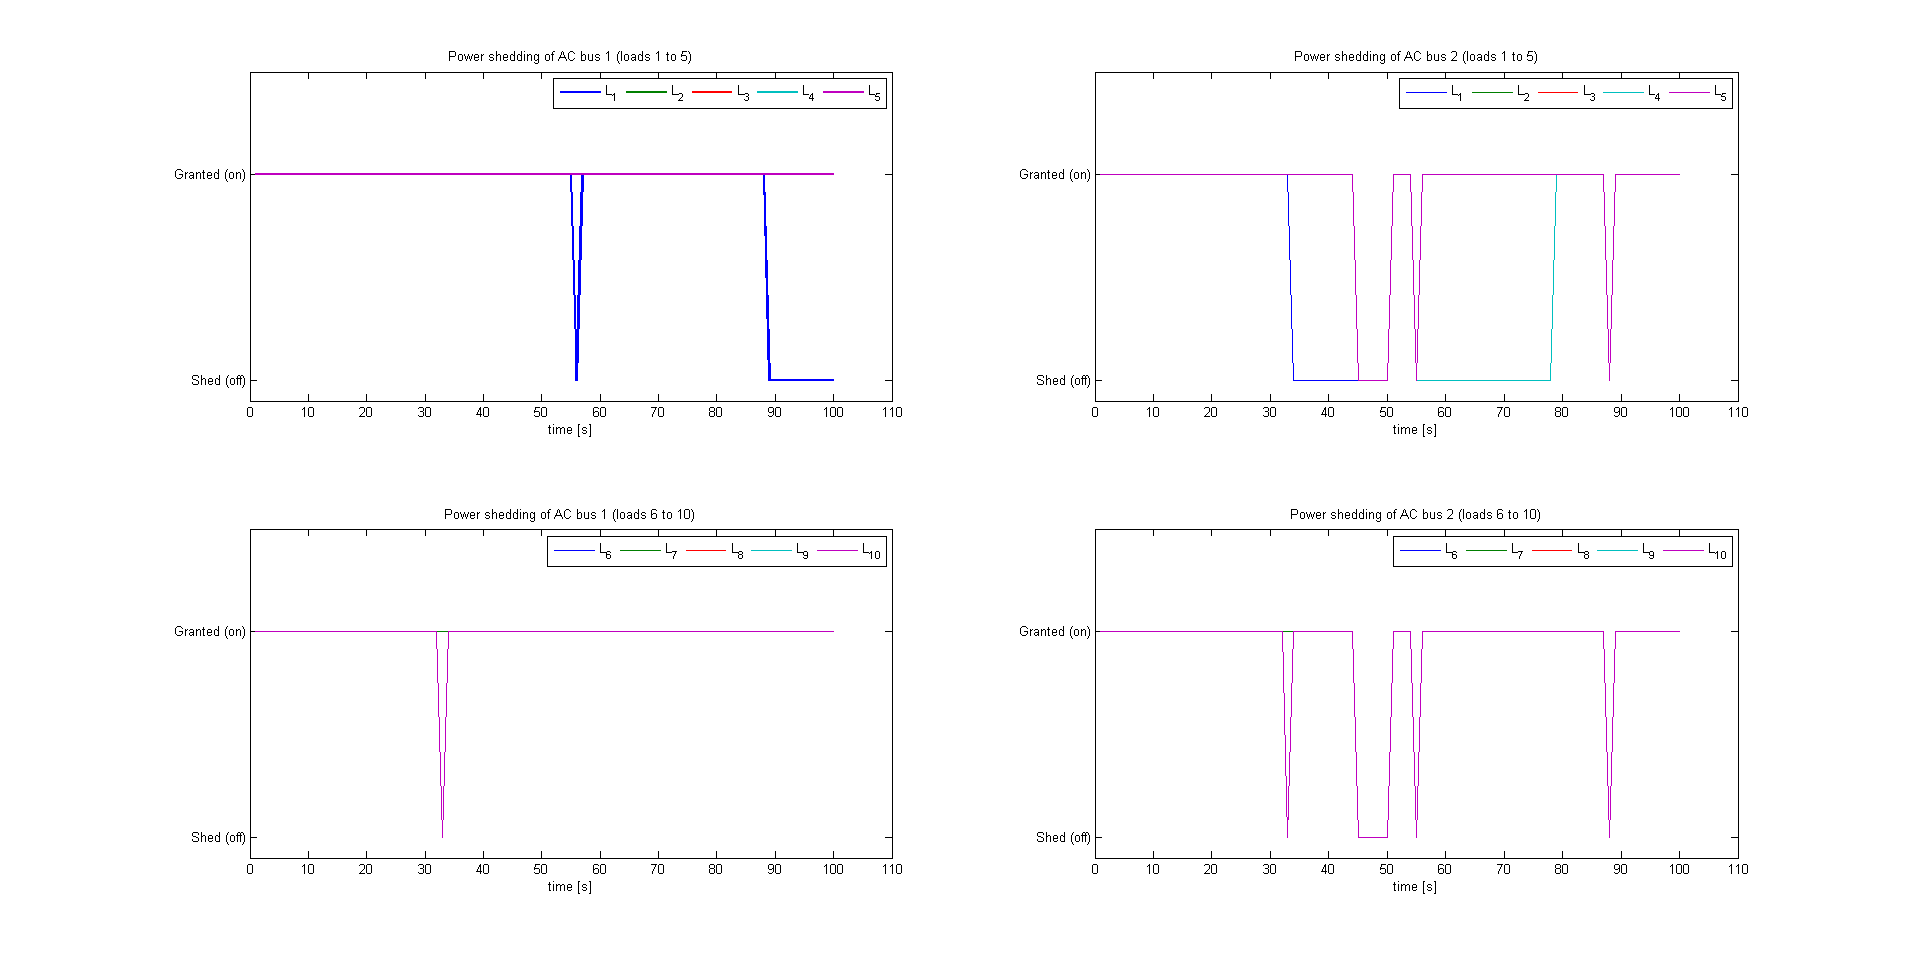
\includegraphics[width=0.9\textwidth]{figures/lsolonefail}
  \caption{\textbf{Hierarchical LMS Load Shedding -- One Generator Failure}. Notice the
  large number of loads dropped from time 45 to 50 before the Optimizing LMS can reoptimize.}
  \label{fig:lsolonefail}
\end{figure*}

\subsection{Unexpected Power Spikes}
\label{sec:power-spikes-simulation}
%The Optimizing LMS performs a live optimization using historical data for load power requests from previous flights. 
%Due to the nature of the optimization problem, it is impossible to program the optimization problem with live data. 
As we showed in Section~\ref{sec:power-spike-example}, it is possible for the Optimizing LMS to provide unsafe advice if there is a power spike. 
More specifically, due to the Optimizing LMS's dependence on historical data, the Optimizing LMS can generate a load shedding configuration that draws more power than the generators can produce. 
We now simulate such a failure case and show that the LL-LMS performs the required adjustment to keep the system in a safe state. 
For this experiment, the Optimizing LMS is given the historical power loads in Figure~\ref{fig:preqnofail}. 
However, the actual power loads for this simulation is shown in Figure~\ref{fig:preqpwrspike}. 
Without the LL-LMS, the Optimizing LMS would use the load shedding configuration seen in Figure~\ref{fig:lshlnofail}. 
Notice that there is a power spike from time 10 to 40 that the historical data does not account for and thus the Optimizing LMS is unaware of. 
As a result, its load shedding configuration would overload the power generator. 
Because we have a LL-LMS, we are able to keep the system in a safe configuration.
Figure~\ref{fig:lsolpwrspike} shows that the LL-LMS detects that the Optimizing LMS's configuration overloads some generators, and the LL-LMS applies the priority tables to shed some loads during this time interval.

\begin{figure}[htb]
  \centering
  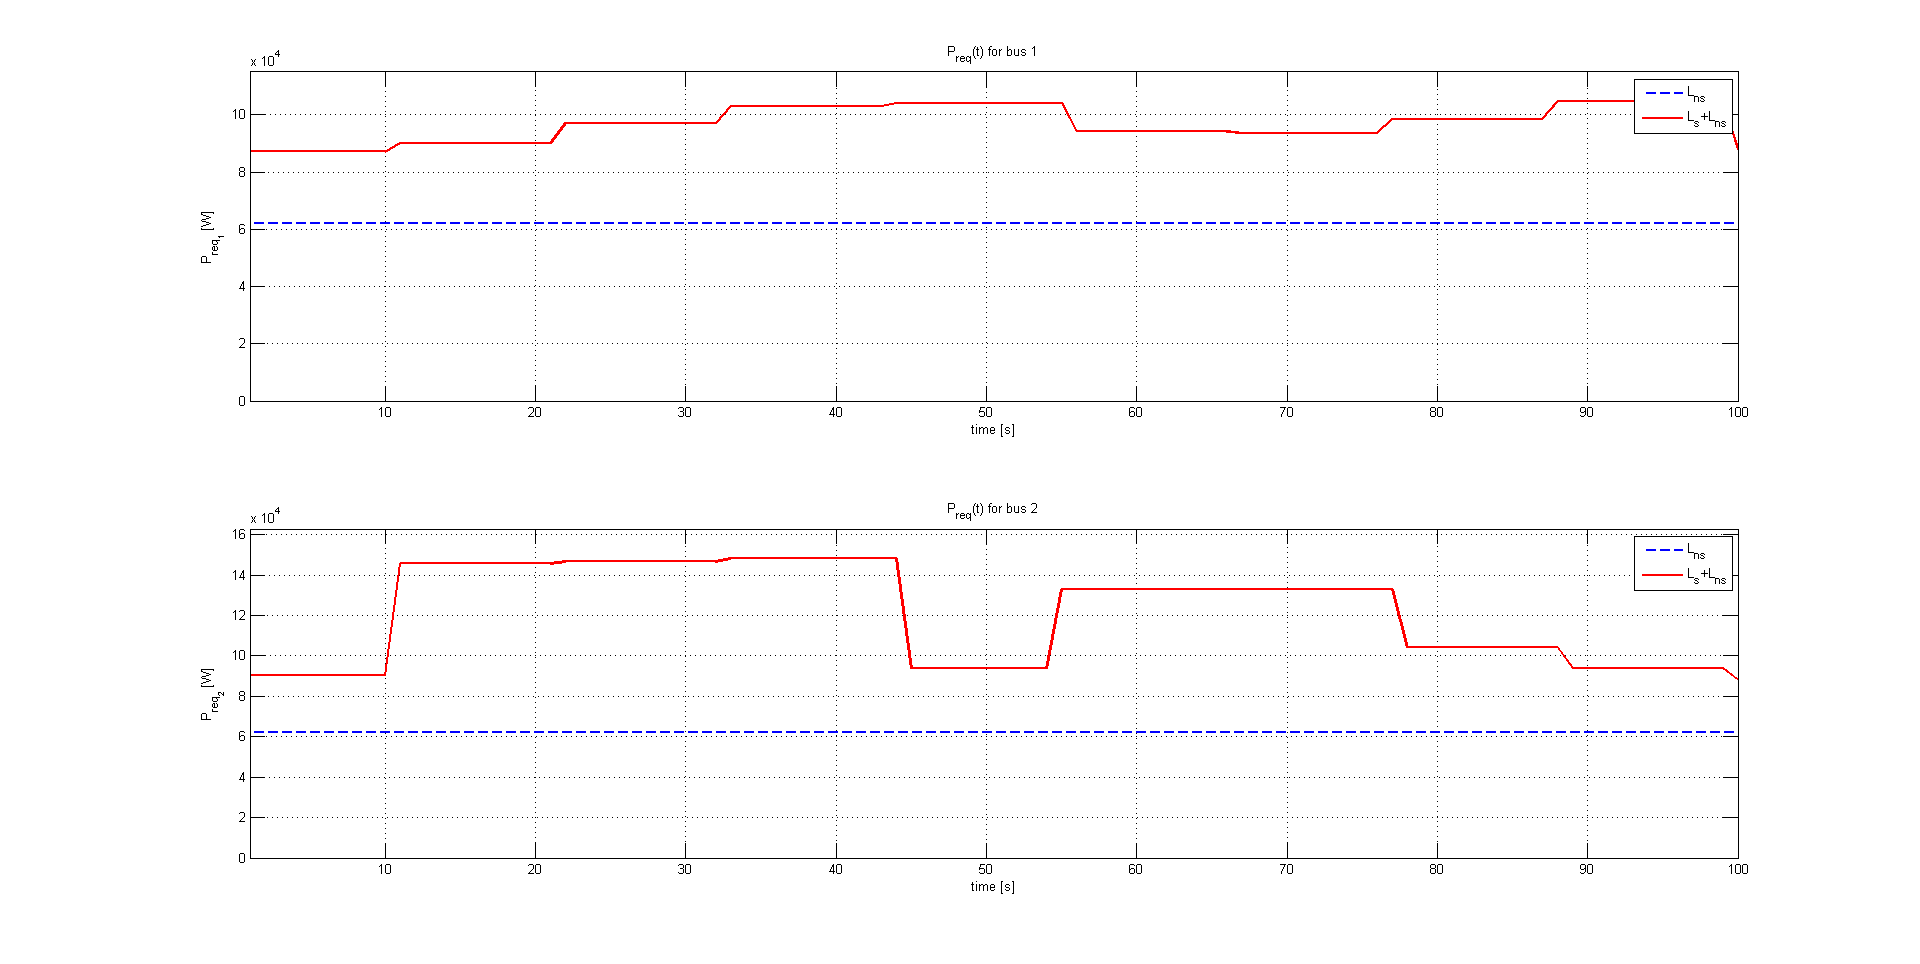
\includegraphics[width=0.9\columnwidth]{figures/preqpwrspike}
  \caption{\textbf{Actual Power Request for Section~\ref{sec:power-spikes-simulation}}. Notice the difference between this power
  request and the power request expected by the historical data in 
  Figure~\ref{fig:preqnofail}. In particular, there is a large power spike from time 10
  to 40 that is not accounted for in the historical data.}
  \label{fig:preqpwrspike}
\end{figure}
\begin{figure*}[hp]
  \centering
  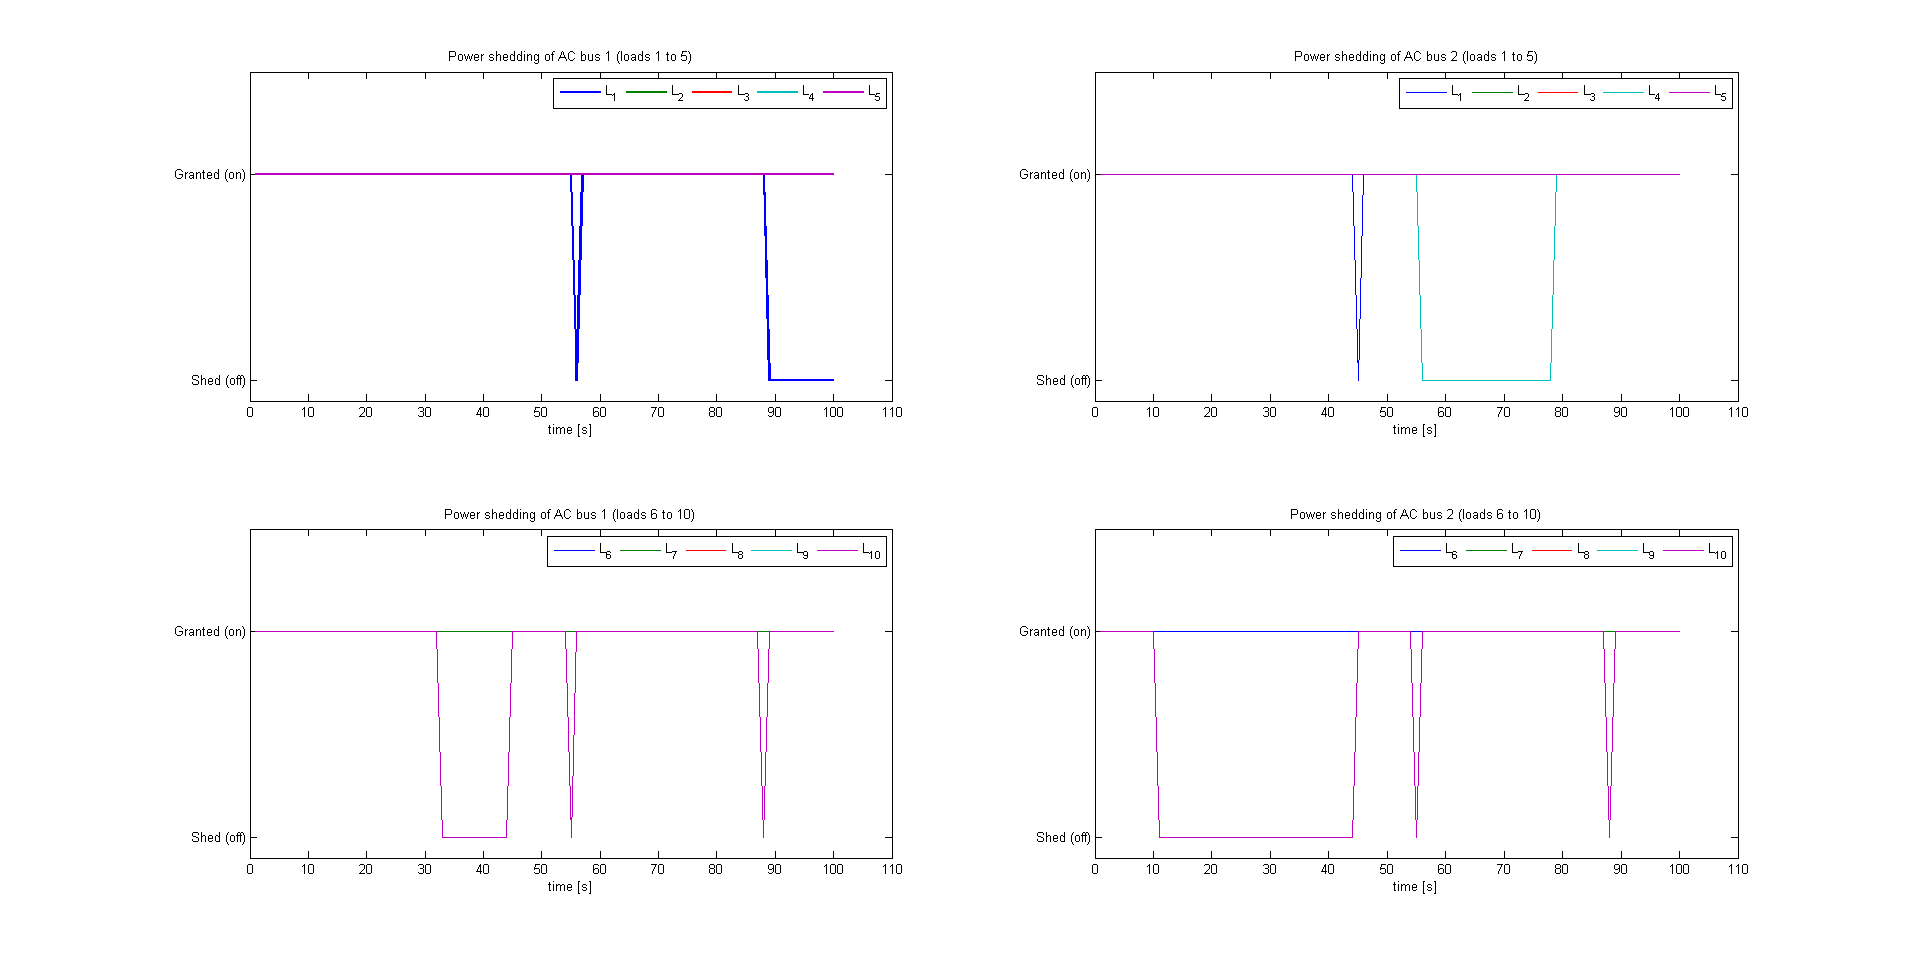
\includegraphics[width=0.9\textwidth]{figures/lsolpwrspike}
  \caption{\textbf{Hierarchical LMS Load Shedding -- Power Spike} Whenever possible the LL-LMS will
  use the advice from the Optimizing LMS. The only time it ignores the advice from the Optimizaing LMS is
  from time 10 to 40 when there is a power spike that the Optimizing LMS is not aware of.}
  \label{fig:lsolpwrspike}
\end{figure*}

\section{Conclusions and Future Work}
We presented a Hierarchical load management system (LMS) for aircraft EPS.
Our Hierarchical LMS minimizes load shedding and optimizes generator assignment when the loads are predicted appropriately, and the Hierarchical LMS reverts to simple priority tables during unexpected EPS loads or failures.
We described the interface and interaction between the two controllers in the Hierarchical LMS, and we showed the intuition and effectiveness of our controller through numerical examples and simulation experiments.

The present paper motivates several avenues for future work.
First, in real-world scenarios, the Optimizing LMS may provide more relevant advice if it has more access to the live data. 
Strategies for fusing the live data with the historical data for use in the Optimizing LMS would be a valuable contribution.
Further, finding ways to reduce the computational complexity of the Optimizing LMS would allow the LL-LMS to request advice from the Optimizing LMS more frequently.
These future work directions would ideally reduce the likelihood that the Hierarchical LMS falls back on the LL-LMS and its pure priority tables, thus increasing the amount of time that the system runs in an optimal configuration.

\section*{Acknowledgments}
This work was supported in part by the US Department of Defense (DoD) through the National Defense Science \& Engineering Graduate Fellowship (NDSEG) Program.

\bibliographystyle{abbrv}
\bibliography{bibliography} 

\end{document}
